\documentclass[11pt]{article}
\usepackage[a4paper,margin=2.5cm]{geometry}
\usepackage[utf8]{inputenc}
\usepackage[T1]{fontenc}
\usepackage{amsmath,amssymb,amsthm,bm}
\usepackage{booktabs}
\usepackage{graphicx}
\usepackage{enumitem}
\usepackage{accents}
\usepackage[round]{natbib}
\usepackage[hidelinks]{hyperref}
\setlist{itemsep=2pt, parsep=0pt, topsep=4pt}
\linespread{1.15}

\DeclareRobustCommand{\dbtilde}[1]{\accentset{\approx}{#1}}
\renewcommand{\vec}[1]{\boldsymbol{#1}}
\newcommand{\E}{\mathbb{E}}
\newcommand{\Z}{\mathbb{Z}}
\newcommand{\N}{\mathbb{N}_0}
\newcommand{\R}{\mathcal{R}}
\newcommand{\Ct}{\widetilde{C}}
\newcommand{\Cq}{\dbtilde{C}}

\newtheorem{theorem}{Theorem}
\newtheorem{lemma}{Lemma}
\newtheorem{proposition}{Proposition}
\newtheorem{corollary}{Corollary}
\theoremstyle{definition}
\newtheorem{assumption}{Assumption}
\newtheorem{remark}{Remark}
\newtheorem{example}{Counterexample}

\title{Structure of the optimal policy of the two-location non-stationary stochastic lot-sizing problem with lateral transshipment}
\author{Working note, 11 November 2026}
\date{}

\begin{document}
\maketitle

\begin{abstract}
\noindent We study the optimal policy of the two-location lot-sizing problem with proactive lateral transshipment, fixed and unit costs on transshipping and on reordering, and non-stationary stochastic demand. We prove that an optimal policy exists and that it is deterministic and Markov. We then prove a structure theorem. The reorder decision is described by one pair of reorder-up-to levels and two reorder-up-to curves in every period. The transshipment decision is described by two transshipment levels on every line of constant total inventory. A transshipment is never followed by reorders at both locations, and the location that ships reorders in the same period only if the fixed reorder cost covers the cost of the transshipment. In the last period the two locations follow independent $(s,S)$ policies. In the earlier periods a location need not reorder below a threshold of its own inventory. We give a sufficient condition for a threshold and a two-period counterexample with Poisson demand, and we explain the mechanism behind it. The threshold property holds in all 336 instances that follow the test beds of the manuscript. We also show by counterexamples that the value function is not $K$-convex and that the transshipment regions are not separated by monotone switching curves. All proved statements are checked numerically on the 336 instances.
\end{abstract}

\section{Introduction}

The manuscript formulates the problem as the stochastic dynamic program SDP-1 and proves that it is equivalent to the two-stage program SDP-2. This note asks what the optimal policy looks like. Three results are known for neighbouring problems. A single location with a fixed reorder cost follows an $(s,S)$ policy, and the proof of \citet{scarf1959optimality} rests on the $K$-convexity of the value function. Two locations with unit costs only follow a policy with switching curves. \citet{abouee2015optimal} prove this for lost sales by convexity, and \citet{xu2023optimal} prove it for backorders by $L^{\natural}$-convexity. With a fixed cost on both actions these properties are not available, and Section~\ref{sec:false} shows that they fail in our problem.

The note proceeds as follows. Section~\ref{sec:literature} reviews the related literature. Section~\ref{sec:model} states the model and the assumptions. Section~\ref{sec:existence} proves that an optimal policy exists. Section~\ref{sec:lemmas} proves five lemmas, and Section~\ref{sec:theorem} combines them into the structure theorem. Section~\ref{sec:threshold} treats the threshold property, with a sufficient condition and a counterexample. Section~\ref{sec:false} lists the properties that do not hold. Section~\ref{sec:numerics} reports the numerical tests.

Every statement called a lemma, a theorem or a proposition is proved in full. Every counterexample is computed numerically, and its margins are far above rounding. Every statement called an observation or an open question is supported by computation only.

\section{Related literature}\label{sec:literature}

Three groups of papers are close to this note. The first characterises the optimal policy when replenishment and transshipment carry unit costs only. The second adds fixed costs to transshipment models but does not characterise the optimal policy over several periods. The third studies the structure of optimal policies under fixed costs in problems without transshipment.

\paragraph{Replenishment and transshipment with unit costs.}
\citet{gross1963centralized} solves the problem with two locations and a single period, and \citet{das1975supply} and \citet{karmarkar1977one} extend the single-period analysis. \citet{karmarkar1981multiperiod} treats several periods and several locations with backorders and proportional costs. He shows that every period has the form of a single-period problem with a convex cost function. The optimal policy has a region of no transactions, and a base-stock vector is optimal when the starting stock is low at every location. \citet{abouee2015optimal} study two locations with lost sales and unit costs. They prove that four switching curves divide the states into eight regions, and they call the result an order-up-to-curve policy. Their conclusion names the case with backorders as an open direction. \citet{xu2023optimal} solve this case. They show that the cost function is $L^{\natural}$-convex, and they describe the optimal policy by five switching curves that are monotone in the state. They state that their paper is the first full characterisation for several periods, two locations and backorders.

The same line of work covers transshipments that take place after the demand is known. \citet{robinson1990optimal} proves that a base-stock policy is optimal for several locations and several periods, and \citet{archibald1997optimal} characterise an optimal policy for two depots with stock transfer. \citet{hu2008optimal} and \citet{yang2007capacitated} characterise the optimal policy for two production locations with uncertain and with limited capacity. \citet{li2014multimodularity} and \citet{chen2015new} obtain such results from multimodularity and from $L^{\natural}$-convexity, and \citet{van2019optimal} describe the optimal transshipment policy with several demand classes by switching curves. \citet{xu2023optimal} compare the methods of these papers. They are convexity, the concavity of a profit function, multimodularity and $L^{\natural}$-convexity. The three models with proactive transshipment over several periods have unit costs only.

\paragraph{Fixed costs in transshipment models.}
\citet{allen1961redistribution} redistributes stock among locations within one delivery interval at a cost per shipment and without replenishment. \citet{herer1999lateral} analyse a single period with two locations, a fixed replenishment cost at each location and a further cost of a common replenishment. The transshipment follows the demand, and they derive the form and several properties of the optimal policies. \citet{noham2014single} add a fixed transshipment cost to the single-period problem with two retailers, again with the transshipment after the demand. \citet{liang2014inventory} study setup costs for transshipment under a demand distribution with three points. \citet{herer2001dynamic} and \citet{herer2003optimal} keep fixed costs over several periods but take the demand as deterministic. \citet{zhou2023replenishment} consider a fixed order cost in a periodic-review system. The retailers reorder together at a common interval, and the authors choose the interval, the order-up-to levels and the time of the transshipment for the long-run average cost. The manuscript has fixed and unit costs on both actions, backorders and non-stationary demand over several periods. It computes the optimal policy and a near-optimal policy, and it does not describe the structure of either. We found no paper that characterises the optimal policy over several periods with stochastic demand when the reorder or the transshipment carries a fixed cost.

\paragraph{Fixed costs and the structure of optimal policies.}
\citet{scarf1959optimality} proves that an $(s,S)$ policy is optimal for a single location, and the proof introduces $K$-convexity. \citet{perera2023survey} survey the work that followed for discrete time. Their survey contains no model with transshipment. Three parts of this literature are close to our problem.

The first part has several products. \citet{johnson1967optimality} considers one fixed cost for any order and proves that the optimal policy reorders up to a level $S$ from the states of a region $\sigma$. This is the $(\sigma,S)$ policy. \citet{kalin1980optimality} gives further conditions and describes the region without orders, and \citet{gallego2005k} generalise $K$-convexity to several dimensions. \citet{perera2023survey} note that only problems with a common fixed cost have been studied. They add that the optimality of the $(\sigma,S)$ policy for every starting inventory has remained open, because $K$-convexity in several dimensions is not enough. \citet{firouzi2014two} allow a separate fixed cost for each of two products but at most one order per period. \citet{kong2024dynamic} combine a common and a separate fixed cost and prove a policy with two regions and one level when the demands increase stochastically over time. The second stage of our problem has a separate fixed cost $K$ at each location. Without transshipment the two locations separate, and each follows an $(s,S)$ policy. The transshipment of the later periods links them, and Counterexample~\ref{ex:threshold} shows that this link removes the threshold.

The second part has fixed costs in two directions. \citet{neave1970stochastic} studies the cash balance problem with a fixed and a proportional cost for increases and for decreases. He shows by an example that a simple policy of the two-sided $(s,S)$ type is not optimal in general. \citet{chen2009new} characterise the optimal policy of this problem by symmetric $K$-convexity, and \citet{ye2007optimal} and \citet{semple2007note} characterise the optimal policy for capacity adjustments with fixed costs in both directions by generalised notions of concavity. The first stage of our problem is of this kind on every line of constant total inventory, with the fixed cost $R$ in both directions.

The third part gives partial characterisations. \citet{shaoxiang1996xy} add a capacity to the single-location problem with a fixed cost. They show that the modified $(s,S)$ policy is not optimal in general. Below a level $X$ the optimal policy orders up to capacity, and above a level $Y$ it does not order. Between the two levels the pattern differs from problem to problem. \citet{gallego2000capacitated} specify the optimal policy of this problem completely for some parameters and partially for the others. \citet{porteus1971optimality} introduces quasi-$K$-convex functions for generalised $(s,S)$ policies, and condition~\eqref{eq:Q} of Section~\ref{sec:threshold} is a condition of this kind.

\paragraph{Position of this note.}
Table~\ref{tab:position} compares this note with the three closest papers. Our model is closest to the backorder model of \citet{xu2023optimal}. It differs in the fixed costs $K$ and $R$, in the order of the two decisions and in the demand. In our model the transshipment precedes the reorders, and the demands are independent and take integer values. The fixed costs remove the convexity on which the three characterisations rest. This note therefore gives a partial characterisation in the sense of \citet{shaoxiang1996xy} and \citet{gallego2000capacitated}. Theorem~\ref{thm:structure} gives the targets of every action and the combinations of actions that can occur. Sections~\ref{sec:threshold} and \ref{sec:false} show by counterexamples that the regions are not bounded by thresholds or by monotone curves in general. To the best of our knowledge this is the first description of the optimal policy of a problem with proactive transshipment, several periods and fixed costs.

\begin{table}[h]
\centering
\small
\caption{This note and the three closest papers.}\label{tab:position}
\begin{tabular}{p{2.9cm}p{1.9cm}p{2.0cm}p{2.4cm}p{4.3cm}}
\toprule
Paper & Unmet demand & Costs & Property used & Description of the optimal policy \\
\midrule
\citet{karmarkar1981multiperiod} & backorders & proportional & convexity & region of no transactions, base-stock vector \\
\citet{abouee2015optimal} & lost sales & unit & convexity & four switching curves, eight regions \\
\citet{xu2023optimal} & backorders, lost sales & unit & $L^{\natural}$-convexity & five monotone switching curves \\
This note & backorders & fixed and unit & exchange of actions & one point, two curves and two levels on every line as targets, five types of action \\
\bottomrule
\end{tabular}
\end{table}

\section{Model and assumptions}\label{sec:model}

We use the notation of the manuscript. There are two locations $j=1,2$ and periods $t=1,\ldots,T$. The state at the start of period $t$ is the pair of inventory levels $\vec{i}=\langle i^1,i^2\rangle\in\Z^2$, and a negative level is a backorder. The events of a period occur in the following order.
\begin{enumerate}
\item A transshipment $W_t\in\R(\vec{i})=\{W\in\Z:\ -\max\{0,i^2\}\le W\le \max\{0,i^1\}\}$ is made. A positive $W_t$ moves $W_t$ units from location~1 to location~2, and a negative $W_t$ moves $|W_t|$ units from location~2 to location~1. Only stock on hand can be moved. The post-transshipment state is $\tilde{\vec{i}}=\langle i^1-W_t,\ i^2+W_t\rangle$.
\item Each location reorders $Q^j_t\in\N$ units from the warehouse. Delivery is immediate. The levels after reordering are $\vec{y}=\tilde{\vec{i}}+\vec{q}_t$ with $\vec{q}_t=\langle Q^1_t,Q^2_t\rangle$.
\item The demands $\vec{d}_t=\langle d^1_t,d^2_t\rangle$ occur, and the next state is $\vec{y}-\vec{d}_t$.
\end{enumerate}
The transshipment cost is $u(w)=R+vw$ for $w>0$ with $u(0)=0$. The reorder cost is $c(Q)=K+zQ$ for $Q>0$ with $c(0)=0$. The expected holding and backorder cost of location $j$ in period $t$ at the level $y$ is
\[
\ell^j_t(y)=\E\big[h\max\{0,y-d^j_t\}+b\max\{0,d^j_t-y\}\big],
\qquad L_t(\vec{y})=\ell^1_t(y^1)+\ell^2_t(y^2).
\]
The cost of the action $a=(W,Q^1,Q^2)$ in state $\vec{i}$ and period $t$ is $r_t(\vec{i},a)=u(|W|)+c(Q^1)+c(Q^2)+L_t(\vec{y})$.

\begin{assumption}\label{ass:demand}
The demands $d^j_t$ are mutually independent, take values in $\N$ and have finite means $\mu^j_t$.
\end{assumption}

\begin{assumption}\label{ass:cost}
$K>0$, $R>0$, $h>0$ and $0<v\le z<b$.
\end{assumption}

Assumption~\ref{ass:demand} covers Poisson demand and the discretised normal demand of the manuscript. Assumption~\ref{ass:cost} holds in both test beds of the manuscript. The condition $z<b$ says that reordering a unit is cheaper than backordering it for one period. The condition $v\le z$ says that moving a unit between the locations costs no more than buying it.

A policy $\pi=(\pi_1,\ldots,\pi_T)$ chooses in period $t$ a probability distribution $\pi_t(\cdot\mid\eta_t)$ on the set of actions $\R(\vec{i}_t)\times\N^2$ as a function of the history $\eta_t=(\vec{i}_1,a_1,\ldots,\vec{i}_{t-1},a_{t-1},\vec{i}_t)$. Its expected total cost from the opening state $\vec{i}$ is $J^\pi(\vec{i})=\E^\pi_{\vec{i}}\big[\sum_{t=1}^T r_t(\vec{i}_t,a_t)\big]\in[0,\infty]$. A policy is deterministic and Markov if its action in period $t$ is a function of $\vec{i}_t$ alone. A policy $\pi^*$ is optimal if $J^{\pi^*}(\vec{i})\le J^{\pi}(\vec{i})$ for every policy $\pi$ and every $\vec{i}$.

The two-stage program SDP-2 is the recursion $\Ct_{T+1}\equiv 0$ and, for $t=T,\ldots,1$,
\begin{align}
\Cq_t(\tilde{\vec{i}})&=\min_{\vec{q}\in\N^2}\Big\{c(Q^1)+c(Q^2)+L_t(\tilde{\vec{i}}+\vec{q})+\E\big[\Ct_{t+1}(\tilde{\vec{i}}+\vec{q}-\vec{d}_t)\big]\Big\},\label{eq:second}\\
\Ct_t(\vec{i})&=\min_{W\in\R(\vec{i})}\Big\{u(|W|)+\Cq_t(\langle i^1-W,\ i^2+W\rangle)\Big\}.\label{eq:first}
\end{align}
We call \eqref{eq:first} the first stage and \eqref{eq:second} the second stage.

\section{Existence of an optimal policy}\label{sec:existence}

The set of reorder quantities is infinite, so the minimum in \eqref{eq:second} needs an argument. Lemmas~\ref{lem:bound} and \ref{lem:coercive} are proved together by backward induction on $t$: each uses the other only for the period $t+1$.

\begin{lemma}[Finite values]\label{lem:bound}
Let $m=\max\{h,b\}$, $\alpha_{T+1}=0$ and $\alpha_t=\alpha_{t+1}+m(T-t+1)(\mu^1_t+\mu^2_t)$. For every $t$ and every $\vec{i}\in\Z^2$,
\[
0\le \Ct_t(\vec{i})\le \alpha_t+m(T-t+1)\big(|i^1|+|i^2|\big).
\]
\end{lemma}

\begin{proof}
The bound holds for $t=T+1$. Suppose that it holds for $t+1$. Then $\E[\Ct_{t+1}(\vec{y}-\vec{d}_t)]$ is finite for every $\vec{y}$, because $\E|y^j-d^j_t|\le |y^j|+\mu^j_t$. All costs are non-negative, so $\Ct_t\ge 0$. The action without transshipment and without reorders gives
\[
\Ct_t(\vec{i})\le L_t(\vec{i})+\E\big[\Ct_{t+1}(\vec{i}-\vec{d}_t)\big].
\]
Since $h\max\{0,y-d\}+b\max\{0,d-y\}\le m|y-d|\le m(|y|+d)$, we have $L_t(\vec{i})\le m\sum_j(|i^j|+\mu^j_t)$. The induction hypothesis gives $\E[\Ct_{t+1}(\vec{i}-\vec{d}_t)]\le\alpha_{t+1}+m(T-t)\sum_j(|i^j|+\mu^j_t)$. The sum of the two bounds is the claim.
\end{proof}

For every $t$ define the function
\begin{equation}\label{eq:H}
H_t(\vec{y})=z(y^1+y^2)+L_t(\vec{y})+\E\big[\Ct_{t+1}(\vec{y}-\vec{d}_t)\big],\qquad \vec{y}\in\Z^2 .
\end{equation}
It is the expected cost from period $t$ onwards as a function of the levels after reordering, with the unit reorder cost charged on the levels. By Lemma~\ref{lem:bound} it is finite. Write $N(\vec{x},\vec{y})$ for the number of locations $j$ with $y^j>x^j$. With $\vec{y}=\tilde{\vec{i}}+\vec{q}$ the second stage \eqref{eq:second} becomes
\begin{equation}\label{eq:secondH}
\Cq_t(\tilde{\vec{i}})=-z(\tilde{i}^1+\tilde{i}^2)+\min_{\vec{y}\ge\tilde{\vec{i}}}\Big\{K\,N(\tilde{\vec{i}},\vec{y})+H_t(\vec{y})\Big\}.
\end{equation}

\begin{lemma}[Attainment]\label{lem:coercive}
For every $t$ and every real number $\gamma$ the set $\{\vec{y}\in\Z^2: H_t(\vec{y})\le\gamma\}$ is finite. Hence $H_t$ attains its minimum on every non-empty subset of $\Z^2$, and the minima in \eqref{eq:second} and \eqref{eq:first} are attained.
\end{lemma}

\begin{proof}
Taking expectations in $h\max\{0,y-d\}+b\max\{0,d-y\}\ge h(y-d)$ and in the same expression $\ge b(d-y)$ gives $\ell^j_t(y)\ge\max\{h(y-\mu^j_t),\,b(\mu^j_t-y)\}$. Since $\Ct_{t+1}\ge 0$,
\[
H_t(\vec{y})\ge\sum_{j=1}^2\psi^j_t(y^j),\qquad \psi^j_t(y)=zy+\max\{h(y-\mu^j_t),\,b(\mu^j_t-y)\}.
\]
As $y\to+\infty$, $\psi^j_t(y)\ge(z+h)y-h\mu^j_t\to\infty$ because $h>0$. As $y\to-\infty$, $\psi^j_t(y)\ge(z-b)y+b\mu^j_t\to\infty$ because $z<b$. So each $\psi^j_t$ is bounded below and has finite sublevel sets on $\Z$, and the same holds for $H_t$ on $\Z^2$. A function with finite sublevel sets attains its minimum on every non-empty subset. The minimum in \eqref{eq:secondH} is the minimum of $H_t$ over at most four such subsets, and $\R(\vec{i})$ is finite.
\end{proof}

\begin{theorem}[Existence]\label{thm:existence}
Let Assumptions~\ref{ass:demand} and \ref{ass:cost} hold. For every $t$ and $\vec{i}$ let $W^*_t(\vec{i})$ attain the minimum in \eqref{eq:first}, and for every $\tilde{\vec{i}}$ let $\vec{q}^*_t(\tilde{\vec{i}})$ attain the minimum in \eqref{eq:second}. Let $\pi^*$ be the deterministic Markov policy that in period $t$ and state $\vec{i}$ transships $W^*_t(\vec{i})$ and then reorders $\vec{q}^*_t(\langle i^1-W^*_t(\vec{i}),\,i^2+W^*_t(\vec{i})\rangle)$. Then
\[
J^{\pi^*}(\vec{i})=\Ct_1(\vec{i})=\inf_{\pi}J^{\pi}(\vec{i})<\infty\qquad\text{for every }\vec{i}\in\Z^2 .
\]
So an optimal policy exists, it can be chosen deterministic and Markov, and its expected total cost is the value of SDP-2.
\end{theorem}

\begin{proof}
For a policy $\pi$ and a history $\eta_t$ let $J^\pi_t(\eta_t)\in[0,\infty]$ be the expected cost of $\pi$ over the periods $t,\ldots,T$ given $\eta_t$, with $J^\pi_{T+1}\equiv0$. We show $J^\pi_t(\eta_t)\ge\Ct_t(\vec{i}_t)$ by backward induction. The claim holds for $T+1$. All terms are non-negative, and by Assumption~\ref{ass:demand} the demand $\vec{d}_t$ is independent of $\eta_t$, so
\begin{align*}
J^\pi_t(\eta_t)&=\sum_{a}\pi_t(a\mid\eta_t)\Big\{r_t(\vec{i}_t,a)+\E\big[J^\pi_{t+1}(\eta_t,a,\vec{y}-\vec{d}_t)\big]\Big\}\\
&\ge\sum_{a}\pi_t(a\mid\eta_t)\Big\{r_t(\vec{i}_t,a)+\E\big[\Ct_{t+1}(\vec{y}-\vec{d}_t)\big]\Big\}.
\end{align*}
For every action $a=(W,Q^1,Q^2)$ the term in braces equals $u(|W|)$ plus the objective of \eqref{eq:second} at $\tilde{\vec{i}}=\langle i^1_t-W,\,i^2_t+W\rangle$ and $\vec{q}$. It is therefore at least $u(|W|)+\Cq_t(\tilde{\vec{i}})$, and this is at least $\Ct_t(\vec{i}_t)$ by \eqref{eq:first}. Hence $J^\pi_t(\eta_t)\ge\Ct_t(\vec{i}_t)$. For $\pi^*$ every inequality is an equality, so $J^{\pi^*}_t(\eta_t)=\Ct_t(\vec{i}_t)$. Taking $t=1$ gives the claim, and Lemma~\ref{lem:bound} gives finiteness.
\end{proof}

\begin{remark}
Proposition~1 of the manuscript shows $C_t=\Ct_t$, so the theorem also holds for SDP-1. The proof uses the independence of the demands between periods, non-negative costs, $h>0$ and finite means. The conditions $v\le z$ and $z<b$ are not needed for the existence of an optimal policy. They are used in Section~\ref{sec:lemmas} for the levels that describe it.
\end{remark}

\section{Lemmas on the two stages}\label{sec:lemmas}

\subsection{Second stage: four reorder patterns}

For $\vec{x}\in\Z^2$ define
\[
M^1_t(\vec{x})=\min_{y^1>x^1}H_t(y^1,x^2),\qquad M^2_t(\vec{x})=\min_{y^2>x^2}H_t(x^1,y^2),\qquad M^{12}_t(\vec{x})=\min_{y^1>x^1,\ y^2>x^2}H_t(\vec{y}).
\]
By Lemma~\ref{lem:coercive} these minima exist. Let $\bar{\vec{S}}_t=\langle\bar S^1_t,\bar S^2_t\rangle$ be a minimiser of $H_t$ over $\Z^2$, let $S^1_t(x^2)$ be a minimiser of $H_t(\cdot,x^2)$ over $\Z$ and let $S^2_t(x^1)$ be a minimiser of $H_t(x^1,\cdot)$ over $\Z$.

\begin{lemma}[Reorder patterns and levels]\label{lem:patterns}
For every $t$ and every post-transshipment state $\vec{x}$,
\begin{equation}\label{eq:four}
\Cq_t(\vec{x})+z(x^1+x^2)=\min\big\{H_t(\vec{x}),\ K+M^1_t(\vec{x}),\ K+M^2_t(\vec{x}),\ 2K+M^{12}_t(\vec{x})\big\}.
\end{equation}
The four terms are the costs of the best decision in which no location reorders, location~1 alone reorders, location~2 alone reorders and both reorder. Moreover
\begin{enumerate}[label=(\roman*)]
\item if $x^1<\bar S^1_t$ and $x^2<\bar S^2_t$, then $M^{12}_t(\vec{x})=H_t(\bar{\vec{S}}_t)$: when both locations reorder, they reorder up to $\bar{\vec{S}}_t$;
\item if $x^1<S^1_t(x^2)$, then $M^1_t(\vec{x})=H_t(S^1_t(x^2),x^2)$: when location~1 alone reorders, it reorders up to $S^1_t(x^2)$;
\item if $x^2<S^2_t(x^1)$, then $M^2_t(\vec{x})=H_t(x^1,S^2_t(x^1))$.
\end{enumerate}
\end{lemma}

\begin{proof}
Split the feasible set $\{\vec{y}\ge\vec{x}\}$ of \eqref{eq:secondH} into the four sets on which $N(\vec{x},\vec{y})$ and the reordering locations are fixed. This gives \eqref{eq:four}. In (i) the point $\bar{\vec{S}}_t$ lies in the set $\{y^1>x^1,\ y^2>x^2\}$ and minimises $H_t$ over $\Z^2$, so it minimises $H_t$ over this set. Parts (ii) and (iii) follow in the same way.
\end{proof}

\begin{lemma}[Reduction to one location]\label{lem:reduction}
Fix $t$ and $x^2$ and define $g^1_t(y^1;x^2)=\min\{H_t(y^1,x^2),\ K+M^2_t(y^1,x^2)\}$. This is the cost when location~1 is at the level $y^1$ after reordering and location~2 then decides optimally. In \eqref{eq:four}, the best decision in which location~1 does not reorder costs $g^1_t(x^1;x^2)$, and the best decision in which it reorders costs $K+\min_{y^1>x^1}g^1_t(y^1;x^2)$. Hence location~1 reorders in every optimal decision at $\vec{x}$ if and only if
\begin{equation}\label{eq:reorder1}
g^1_t(x^1;x^2)>K+\min_{y^1>x^1}g^1_t(y^1;x^2).
\end{equation}
The same holds for location~2 with $g^2_t(y^2;x^1)=\min\{H_t(x^1,y^2),\ K+M^1_t(x^1,y^2)\}$.
\end{lemma}

\begin{proof}
The first claim is the definition of $g^1_t$. For the second, $\min\{K+M^1_t(\vec{x}),\,2K+M^{12}_t(\vec{x})\}=K+\min_{y^1>x^1}\min\{H_t(y^1,x^2),\,K+\min_{y^2>x^2}H_t(y^1,y^2)\}$, and the inner minimum is $g^1_t(y^1;x^2)$.
\end{proof}

Given the inventory of the other location, each location therefore faces a single-location problem with the cost function $g^j_t$. The function depends on the other location, and so do the levels.

\subsection{Combinations of a transshipment with reorders}

Two actions at the same state with the same levels $\vec{y}$ after reordering have the same expected holding, backorder and future costs. They differ only in $u(|W|)+c(Q^1)+c(Q^2)$.

\begin{lemma}[Exchange]\label{lem:exchange}
Let $(W,Q^1,Q^2)$ be an optimal action at some state in some period with $W>0$. Then
\begin{enumerate}[label=(\roman*)]
\item $Q^1=0$ or $Q^2=0$: a transshipment is not followed by reorders at both locations;
\item if the sender reorders, $Q^1>0$, then $Q^1>W$ and $K\ge R+vW$.
\end{enumerate}
The same holds for $W<0$ with the two locations exchanged and $W$ replaced by $|W|$.
\end{lemma}

\begin{proof}
Let the state be $\vec{i}$, so that $0<W\le i^1$ and $\vec{y}=\langle i^1-W+Q^1,\ i^2+W+Q^2\rangle$. Every alternative below is feasible and reaches the same $\vec{y}$.

(i) Suppose $Q^1>0$ and $Q^2>0$. If $Q^1>W$, the action $(0,\,Q^1-W,\,Q^2+W)$ costs $R+vW$ less. If $Q^1=W$, the action $(0,\,0,\,Q^2+W)$ costs $R+vW+K$ less. If $Q^1<W$, the action $(W-Q^1,\,0,\,Q^2+Q^1)$ costs $K+vQ^1$ less. Each saving is positive, which contradicts optimality.

(ii) Suppose $Q^1>0$, and so $Q^2=0$ by (i). If $Q^1>W$, the action $(0,\,Q^1-W,\,W)$ changes the cost by $K-(R+vW)$, so optimality requires $K\ge R+vW$. If $Q^1=W$, the action $(0,0,W)$ costs $R+vW$ less. If $Q^1<W$, the action $(W-Q^1,\,0,\,Q^1)$ costs $vQ^1$ less. The last two cases contradict optimality.
\end{proof}

\begin{corollary}\label{cor:types}
Every optimal action is of one of five types: no action; reorders without transshipment; a transshipment without reorders; a transshipment after which the receiver alone reorders; a transshipment of $|W|$ units after which the sender alone reorders more than $|W|$ units. The last type requires $K\ge R+v|W|$. If $K<R+v$, it never occurs.
\end{corollary}

In the last type the sender reorders for both locations in the same period. It passes on stock and replaces it at once. This saves the fixed reorder cost of the receiver at the price of a transshipment.

\subsection{First stage: one line of constant total inventory}

A transshipment leaves the total inventory $n=i^1+i^2$ unchanged. For $n\in\Z$ define on the line $\{\langle x,\,n-x\rangle\}$
\[
G_{t,n}(x)=\Cq_t(\langle x,\,n-x\rangle),\qquad \varphi^+_{t,n}(x)=G_{t,n}(x)-vx,\qquad \varphi^-_{t,n}(x)=G_{t,n}(x)+vx .
\]

\begin{lemma}[Transshipment levels]\label{lem:line}
For every $t$, every $n$ and every state $\vec{i}=\langle i^1,\,n-i^1\rangle$,
\begin{equation}\label{eq:line}
\Ct_t(\vec{i})=\min\Big\{G_{t,n}(i^1),\ \ R+vi^1+\min_{0\le x<i^1}\varphi^+_{t,n}(x),\ \ R-vi^1+\min_{i^1<x\le n}\varphi^-_{t,n}(x)\Big\},
\end{equation}
where a minimum over an empty set is $+\infty$. The three terms are no transshipment, the best transshipment from location~1 to location~2 and the best transshipment from location~2 to location~1, and $x$ is the inventory of location~1 after the transshipment. Moreover
\begin{enumerate}[label=(\roman*)]
\item $\varphi^+_{t,n}$ has a minimiser $D^+_t(n)$ over $\{x\ge0\}$, and $\varphi^-_{t,n}$ has a minimiser $D^-_t(n)$ over $\{x\le n\}$;
\item for $i^1>D^+_t(n)$ the best transshipment from location~1 to location~2 brings location~1 down to $D^+_t(n)$, and it is cheaper than no transshipment if and only if $\varphi^+_{t,n}(i^1)-\varphi^+_{t,n}(D^+_t(n))>R$;
\item for $i^1<D^-_t(n)$ the best transshipment from location~2 to location~1 brings location~1 up to $D^-_t(n)$, and it is cheaper than no transshipment if and only if $\varphi^-_{t,n}(i^1)-\varphi^-_{t,n}(D^-_t(n))>R$;
\item $D^-_t(n)\le D^+_t(n)$.
\end{enumerate}
\end{lemma}

\begin{proof}
A transshipment $W>0$ is feasible if and only if $1\le W\le i^1$. With $x=i^1-W$ this is $0\le x<i^1$, and its cost is $R+v(i^1-x)+G_{t,n}(x)=R+vi^1+\varphi^+_{t,n}(x)$. A transshipment $W<0$ is feasible if and only if $1\le -W\le n-i^1$. With $x=i^1-W$ this is $i^1<x\le n$, and its cost is $R+v(x-i^1)+G_{t,n}(x)=R-vi^1+\varphi^-_{t,n}(x)$. This proves \eqref{eq:line}.

(i) Drop the fixed costs and the future cost in \eqref{eq:second}: $\Cq_t(\vec{x})\ge\sum_j\theta^j_t(x^j)$ with $\theta^j_t(x)=\min_{Q\ge0}\{zQ+\max\{h(x+Q-\mu^j_t),\,b(\mu^j_t-x-Q)\}\}$. Clearly $\theta^j_t(x)\ge h(x-\mu^j_t)$. For $Q\le\mu^j_t-x$ we have $zQ+b(\mu^j_t-x-Q)\ge z(\mu^j_t-x)$ because $z<b$, and for $Q>\mu^j_t-x$ we have $zQ>z(\mu^j_t-x)$, so $\theta^j_t(x)\ge z(\mu^j_t-x)$. Hence
\[
\varphi^+_{t,n}(x)\ge h(x-\mu^1_t)+z(\mu^2_t-n+x)-vx=(h+z-v)x+\text{constant},
\]
which tends to infinity as $x\to+\infty$ because $h>0$ and $v\le z$. The set $\{x\ge0\}$ is bounded below, so a minimiser exists. In the same way $\varphi^-_{t,n}(x)\ge z(\mu^1_t-x)+h(n-x-\mu^2_t)+vx$ tends to infinity as $x\to-\infty$.

(ii) For $i^1>D^+_t(n)$ the point $D^+_t(n)$ lies in $\{0\le x<i^1\}$, so it attains the inner minimum of the second term of \eqref{eq:line}. The second term is smaller than the first if and only if $R+vi^1+\varphi^+_{t,n}(D^+_t(n))<G_{t,n}(i^1)$, which is the stated inequality. Part (iii) is symmetric.

(iv) If $D^-_t(n)<0$ or $D^+_t(n)>n$ the claim holds because $D^+_t(n)\ge0$ and $D^-_t(n)\le n$. Otherwise both points lie in $\{0\le x\le n\}$, so $\varphi^+_{t,n}(D^+_t)\le\varphi^+_{t,n}(D^-_t)$ and $\varphi^-_{t,n}(D^-_t)\le\varphi^-_{t,n}(D^+_t)$. Adding the two inequalities gives $2v\,(D^-_t(n)-D^+_t(n))\le0$, and $v>0$.
\end{proof}

A state with $i^1\le D^+_t(n)$ can still ship from location~1 to location~2. Its target is then a minimiser of $\varphi^+_{t,n}$ over $\{0\le x<i^1\}$, which can be the point $x=0$ at which location~1 ships all its stock.

\subsection{Last period}

\begin{lemma}[Last period]\label{lem:last}
In period $T$ let $f^j(y)=zy+\ell^j_T(y)$, let $S^j_T$ be the smallest minimiser of $f^j$ over $\Z$ and let $s^j_T=\max\{x<S^j_T:\ f^j(x)>K+f^j(S^j_T)\}$. Then the following decision is optimal in the second stage at every state $\vec{x}$: location $j$ reorders up to $S^j_T$ if $x^j\le s^j_T$ and does not reorder otherwise. Each location follows an $(s,S)$ policy that does not depend on the other location.
\end{lemma}

\begin{proof}
Since $\Ct_{T+1}\equiv0$, $H_T(\vec{y})=f^1(y^1)+f^2(y^2)$, and \eqref{eq:secondH} separates into one problem per location, $\min\{f^j(x^j),\ K+\min_{y>x^j}f^j(y)\}$. Each $f^j$ is convex as the sum of a linear function and an expectation of convex functions, and it tends to infinity in both directions by the proof of Lemma~\ref{lem:coercive}. So $f^j$ is non-increasing on $\{y\le S^j_T\}$ and non-decreasing on $\{y\ge S^j_T\}$. For $x\ge S^j_T$, $\min_{y>x}f^j(y)\ge f^j(x)$, and a reorder costs $K$ more than none. For $x<S^j_T$, $\min_{y>x}f^j(y)=f^j(S^j_T)$, and a reorder is cheaper if and only if $f^j(x)>K+f^j(S^j_T)$. The set of these $x$ is non-empty because $f^j$ is unbounded, and it contains every level below one of its elements because $f^j$ is non-increasing there. Its largest element is $s^j_T$.
\end{proof}

\section{Structure of the optimal policy}\label{sec:theorem}

\begin{theorem}[Structure]\label{thm:structure}
Let Assumptions~\ref{ass:demand} and \ref{ass:cost} hold. For every period $t$ there are a point $\bar{\vec{S}}_t\in\Z^2$, two functions $S^1_t,S^2_t:\Z\to\Z$ and two functions $D^+_t,D^-_t:\Z\to\Z$ with $D^-_t(n)\le D^+_t(n)$, all defined from $H_t$ and $\Cq_t$ as in Section~\ref{sec:lemmas}, such that an optimal policy has the following form in period $t$ and state $\vec{i}$ with $n=i^1+i^2$.
\begin{enumerate}[label=(\alph*)]
\item \emph{Transshipment.} The policy compares three alternatives by \eqref{eq:line}: no transshipment, a transshipment from location~1 to location~2 and a transshipment from location~2 to location~1. If $i^1>D^+_t(n)$, a transshipment from location~1 to location~2 brings location~1 down to $D^+_t(n)$, and it is preferred to no transshipment exactly when $\varphi^+_{t,n}(i^1)-\varphi^+_{t,n}(D^+_t(n))>R$. If $i^1<D^-_t(n)$, a transshipment from location~2 to location~1 brings location~1 up to $D^-_t(n)$, and it is preferred to no transshipment exactly when $\varphi^-_{t,n}(i^1)-\varphi^-_{t,n}(D^-_t(n))>R$. In the remaining cases the target of a transshipment is a minimiser of $\varphi^+_{t,n}$ over $\{0\le x<i^1\}$ or of $\varphi^-_{t,n}$ over $\{i^1<x\le n\}$.
\item \emph{Reorders.} At the post-transshipment state $\tilde{\vec{i}}$ the policy chooses the cheapest of the four patterns of \eqref{eq:four}. If both locations reorder and $\tilde{\vec{i}}<\bar{\vec{S}}_t$ in both components, they reorder up to $\bar{\vec{S}}_t$. If location~$j$ alone reorders and $\tilde{i}^j$ lies below $S^j_t$ evaluated at the inventory of the other location, it reorders up to this level. Location~$j$ reorders in every optimal decision if and only if \eqref{eq:reorder1} holds for $g^j_t$.
\item \emph{Combinations.} A transshipment is never followed by reorders at both locations. The sender reorders after a transshipment of $|W|$ units only if it reorders more than $|W|$ units and $K\ge R+v|W|$. If $K<R+v$, only the receiver can reorder after a transshipment.
\item \emph{Last period.} In period $T$ the reorders follow two independent $(s^j_T,S^j_T)$ policies: $S^j_T(\cdot)\equiv S^j_T$, $\bar{\vec{S}}_T=\langle S^1_T,S^2_T\rangle$, and location $j$ reorders if and only if $\tilde{i}^j\le s^j_T$.
\end{enumerate}
\end{theorem}

\begin{proof}
By Theorem~\ref{thm:existence} a policy is optimal if it attains the minima of \eqref{eq:first} and \eqref{eq:second} in every period and state. Part (a) is Lemma~\ref{lem:line}. Part (b) is Lemma~\ref{lem:patterns} together with Lemma~\ref{lem:reduction}. Part (c) is Lemma~\ref{lem:exchange} and Corollary~\ref{cor:types}, which hold for every optimal action. Part (d) is Lemma~\ref{lem:last}.
\end{proof}

The theorem describes the optimal policy by five objects per period. The pair $\bar{\vec{S}}_t$ generalises the reorder-up-to level $S$ of a single location to the case in which both locations reorder. The curves $S^1_t$ and $S^2_t$ are the reorder-up-to levels of a location that reorders alone, and they depend on the inventory of the other location. The levels $D^+_t(n)$ and $D^-_t(n)$ play the same role for the transshipment on each line of constant total inventory, with the fixed cost $R$ in place of $K$. Figure~\ref{fig:levels} shows the five objects for one instance.

\begin{figure}[t]
\centering
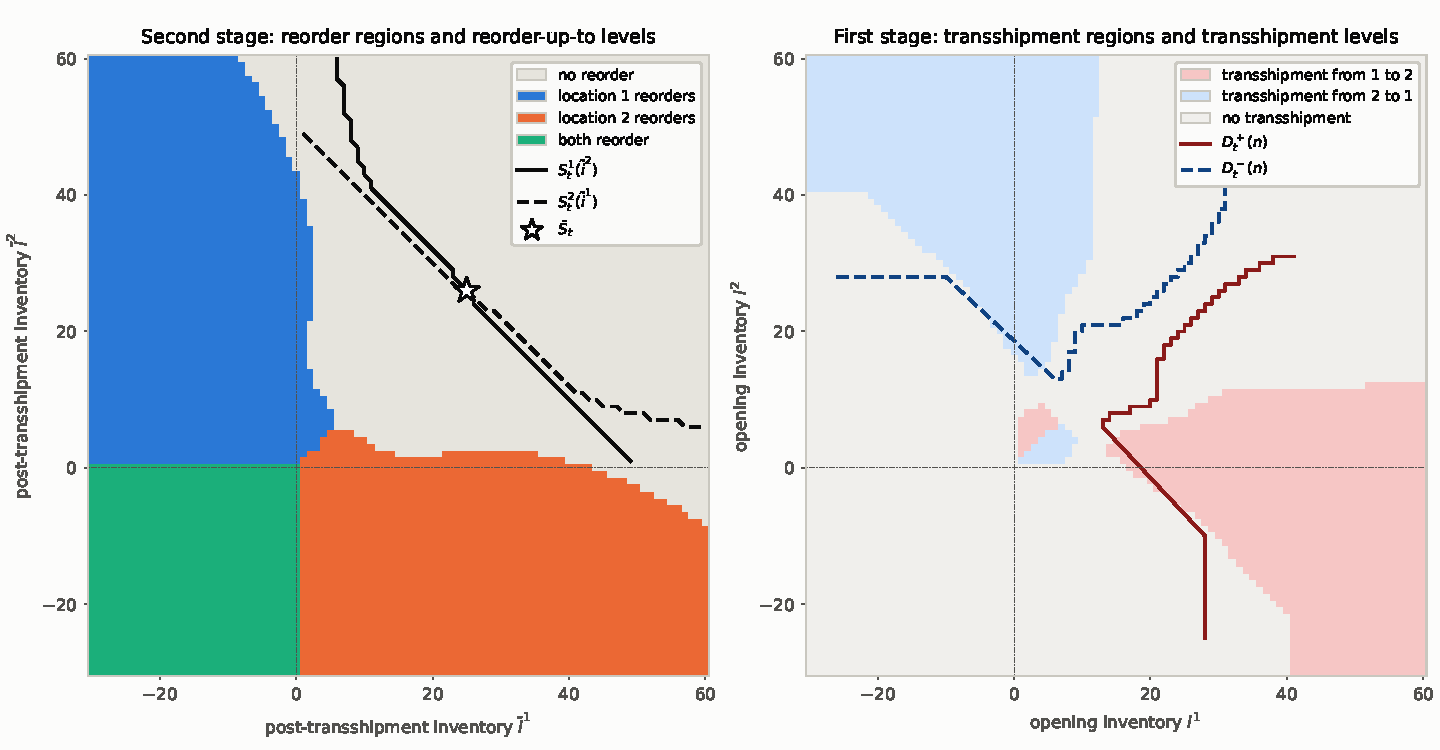
\includegraphics[width=\textwidth]{fig_levels_STAT-STAT_T4_K50_R2.pdf}
\caption{Levels of Theorem~\ref{thm:structure} in period~1 for the pair STAT--STAT with $T=4$, Poisson demand, $K=50$, $R=2$, $z=1$, $v=0.5$, $h=1$ and $b=5$. A level is drawn where the optimal policy uses it.}
\label{fig:levels}
\end{figure}

The theorem does not say that the region in which a location reorders is bounded by a threshold, and it does not say that the states without transshipment form an interval of each line. Both properties fail in general, as Sections~\ref{sec:threshold} and \ref{sec:false} show.

\section{Thresholds}\label{sec:threshold}

In a single-location problem the reorder region is $\{x\le s\}$. The corresponding statement here is that location~1 reorders at $\langle x^1,x^2\rangle$ if and only if $x^1\le s^1_t(x^2)$. By Lemma~\ref{lem:reduction} this is a property of the one-dimensional function $g^1_t(\cdot\,;x^2)$.

\begin{proposition}[Sufficient condition]\label{prop:Q}
Fix $t$ and $x^2$ and write $g=g^1_t(\cdot\,;x^2)$. Suppose that
\begin{equation}\label{eq:Q}\tag{Q}
g(x)\le\max\{g(x'),\ K+g(y)\}\qquad\text{for all integers }x'<x<y .
\end{equation}
Then there is an integer $s^1_t(x^2)$ such that location~1 reorders in every optimal decision at $\langle x^1,x^2\rangle$ if and only if $x^1\le s^1_t(x^2)$.
\end{proposition}

\begin{proof}
Let $A$ be the set of $x$ that satisfy \eqref{eq:reorder1}, that is $g(x)>K+\min_{y>x}g(y)$. Let $x\in A$ and $x'<x$, and let $y^*>x$ attain the minimum. Then $g(x)>K+g(y^*)$, and \eqref{eq:Q} with the triple $x'<x<y^*$ gives $g(x)\le g(x')$. So $g(x')\ge g(x)>K+g(y^*)\ge K+\min_{y>x'}g(y)$ and $x'\in A$. The set $A$ is non-empty: $g(x)\ge\psi^1_t(x)+\min\psi^2_t\to\infty$ as $x\to-\infty$, whereas $K+\min_{y>x}g(y)$ is non-increasing as $x$ decreases. The set $A$ is bounded above: otherwise $A=\Z$, and starting from any point one finds $y_1<y_2<\cdots$ with $g(y_{k+1})<g(y_k)-K$, which contradicts that $g$ is bounded below. So $A=\{x\le s\}$ with $s=\max A$.
\end{proof}

Condition~\eqref{eq:Q} is weaker than $K$-convexity. It only forbids a point whose cost exceeds the cost of a lower point and also exceeds the cost of a higher point by more than $K$. In the last period $g^j_T$ equals the convex function $f^j$ of Lemma~\ref{lem:last} plus a constant, and \eqref{eq:Q} holds. In the earlier periods \eqref{eq:Q} can fail, and so can the threshold property.

\begin{example}[A location does not reorder below a threshold]\label{ex:threshold}
Two periods, Poisson demand, expected demands $(1,30)$ at location~1 and $(1,12)$ at location~2, $K=57$, $R=2$, $z=1$, $v=0.5$, $h=1$ and $b=20$. Assumptions~\ref{ass:demand} and \ref{ass:cost} hold. Table~\ref{tab:threshold} gives the second stage of period~1 at the states $\langle\tilde{i}^1,3\rangle$. Location~1 reorders at $\tilde{i}^1\le2$, does not reorder at $\tilde{i}^1=3$, reorders again at $\tilde{i}^1=4,5,6,7$ and does not reorder at $\tilde{i}^1\ge8$. Whenever it reorders, it reorders up to 50, and location~2 does not reorder. No transshipment is optimal at the opening states $\langle i^1,3\rangle$ with $-1\le i^1\le11$, so these states are reached by the optimal policy.
\end{example}

\begin{table}[h]
\centering
\footnotesize
\setlength{\tabcolsep}{2.6pt}
\caption{Counterexample~\ref{ex:threshold}: cost of the best reorder decision at $\langle\tilde{i}^1,3\rangle$ in period~1 without and with a reorder at location~1.}\label{tab:threshold}
\begin{tabular}{lrrrrrrrrr}
\toprule
$\tilde{i}^1$ & 1 & 2 & 3 & 4 & 5 & 6 & 7 & 8 & 9 \\
\midrule
Without & 197.4030 & 191.8553 & 190.1705 & 189.7735 & 189.6984 & 189.5108 & 187.4096 & 182.0439 & 174.0828 \\
With & 192.6524 & 191.6524 & 190.6524 & 189.6524 & 188.6524 & 187.6524 & 186.6524 & 185.6524 & 184.6524 \\
Difference & 4.7506 & 0.2028 & $-0.4819$ & 0.1211 & 1.0460 & 1.8583 & 0.7571 & $-3.6085$ & $-10.5696$ \\
Reorder at 1 & yes & yes & no & yes & yes & yes & yes & no & no \\
\bottomrule
\end{tabular}
\end{table}

The values of Table~\ref{tab:threshold} are computed with the demand truncated at its $1-10^{-4}$ quantile, as in the manuscript. They are confirmed in two ways. The code of the manuscript returns the same policy and the same costs to four decimals. A separate enumeration of the two-period problem, which shares no code with it, returns the same values, and with the tail of the demand cut at $10^{-12}$ the differences at $\tilde{i}^1=2,\ldots,7$ are $0.2043$, $-0.4821$, $0.1192$, $1.0423$, $1.8538$ and $0.7526$.

The mechanism is the following. Both locations hold enough stock for period~1, and both need stock in period~2. If neither reorders in period~1, both reorder in period~2, for example in the state $\langle2,2\rangle$. If location~1 reorders up to 50 in period~1, it supplies location~2 by a transshipment in period~2. In the state $\langle50,2\rangle$ of period~2, for example, it ships 14 units and neither location reorders. This saves one fixed reorder cost of 57 at the price of the transshipment and of one period of holding. At $\langle3,3\rangle$ the two alternatives are close, and waiting is cheaper by $0.4819$. With one more unit at location~1 the cost with the reorder falls by the unit cost $z=1$, because one unit less is bought. The cost without the reorder falls by less, $0.3970$, $0.0751$ and $0.1876$ from 3 to 6 units, because the additional unit is only held. The reorder is therefore the cheaper alternative from 4 to 7 units. With 8 units or more waiting is cheaper again. In the state $\langle9,2\rangle$ of period~2, for example, location~1 ships its 9 units to location~2 and reorders alone, and this also saves one fixed reorder cost.

The counterexample combines three ingredients. A reorder of one location for both must pay, so $K$ must exceed the cost $R+v|W|$ of the later transshipment plus the holding cost. The other location must not be able to take this role at the same cost, which holds here because the demand of location~1 in period~2 is larger. The fixed reorder cost must lie in the narrow range in which the two alternatives are close. A targeted search of Section~\ref{sec:numerics} finds the same failure for normal demand with $\rho=0.1$, $0.2$ and $0.3$, and it finds no failure when $K\le R+v$.

The thresholds, where they exist, are not monotone in general: in the pair STAT--STAT with $T=4$, $K=50$ and $R=2$ the threshold of location~1 in period~1 takes the values $1,5,4,2,1,2$ at $\tilde{i}^2=2,6,10,14,18,22$.

\section{Properties that do not hold}\label{sec:false}

The following counterexamples are computed with SDP-2 on a range of inventory levels that is wide enough for no demand outcome to be dropped on the states shown. All instances have $T=4$, Poisson demand, $z=1$, $v=0.5$, $h=1$ and $b=5$. The expected demands are $(7,7,7,7)$ for STAT, $(2,5,10,11)$ for LCY1, $(6,13,7,2)$ for LCY2 and $(2,2,2,2)$ for STAT/3. Every difference quoted is larger than $10^{-2}$, far above rounding.

\begin{example}[The states without transshipment are not an interval of a line]\label{ex:interval}
STAT--STAT, $K=50$, $R=2$, period~1, line $n=10$. No transshipment is made at $\langle1,9\rangle$. At $\langle2,8\rangle$, $\langle3,7\rangle$ and $\langle4,6\rangle$ location~1 ships all its stock to location~2 and then reorders. At $\langle5,5\rangle$ to $\langle8,2\rangle$ location~2 ships all its stock to location~1 and then reorders. No transshipment is made at $\langle9,1\rangle$. At $\langle2,8\rangle$ the optimal action is $(W,Q^1,Q^2)=(2,40,0)$ with $\Ct_1=211.395$, against $\Cq_1=212.037$ without transshipment. The location with less stock is the sender, so the directions are not ordered along the line either.
\end{example}

\begin{example}[The same failure in a one-period problem]\label{ex:last}
LCY1--LCY2, $K=50$, $R=2$, period~4, line $n=-1$. No transshipment is made at $\langle9,-10\rangle$. At $\langle10,-11\rangle$ and $\langle11,-12\rangle$ location~1 ships 3 and 4 units. At $\langle12,-13\rangle$ to $\langle15,-16\rangle$ no transshipment is made and location~2 reorders. At $\langle16,-17\rangle$ location~1 ships 9 units. Every transshipment ends at $\tilde{\vec{i}}=\langle7,-8\rangle$, which is the level $D^+_4(-1)=7$ of Theorem~\ref{thm:structure}. The cause is the kink of $\Cq_4$ at the reorder threshold $s^2_4=-12$ of location~2.
\end{example}

\begin{example}[$\Ct_t$ is not $K$-convex]\label{ex:kconv}
STAT--STAT, $K=50$, $R=2$, period~1. $\Ct_1(-1,0)=259.549$, $\Ct_1(0,0)=258.549$ and $\Ct_1(50,0)=122.585$. $K$-convexity in $i^1$ requires $\Ct_1(50,0)+K\ge\Ct_1(0,0)+50\,(\Ct_1(0,0)-\Ct_1(-1,0))=208.549$, but the left-hand side is $172.585$. Stock at location~1 can serve location~2 through a transshipment, so it saves more than one fixed reorder cost.
\end{example}

\begin{example}[$\Cq_t$ is not $K$-convex when $K=R$]\label{ex:kconv2}
STAT--STAT/3, $K=20$, $R=20$, period~1. $\Cq_1(4,11)=116.090$, $\Cq_1(4,12)=119.079$ and $\Cq_1(4,38)=136.713$. $K$-convexity in $\tilde{i}^2$ requires $\Cq_1(4,38)+K\ge\Cq_1(4,12)+26\,(\Cq_1(4,12)-\Cq_1(4,11))=196.800$, but the left-hand side is $156.713$.
\end{example}

\begin{example}[The reorder-up-to level of one location depends on the other]\label{ex:slope}
STAT--STAT, $K=50$, $R=2$, period~1. $S^1_1(\tilde{i}^2)=48,44,40,36,32,28$ at $\tilde{i}^2=2,6,10,14,18,22$, so $S^1_1(\tilde{i}^2)+\tilde{i}^2=50$. The single-location level is 25. The location that reorders raises the total stock of the two locations to twice the single-location level and transships later. With $K=20$ and $R=20$ the level is 21 for $\tilde{i}^2=5,9,\ldots,29$, which is the single-location level.
\end{example}

Counterexamples~\ref{ex:kconv} and \ref{ex:kconv2} explain why the classical proof of the $(s,S)$ policy does not extend: the minimisation over the transshipment in \eqref{eq:first} does not preserve $K$-convexity. Counterexample~\ref{ex:last} shows that the difficulty is not caused by the future, since it appears in the last period.

\section{Numerical tests}\label{sec:numerics}

\subsection{Instances and method}

We test four sets of instances, 336 in total, all with $h=1$.
\begin{itemize}
\item Set A is test bed~II of the manuscript at $T=4$: $K\in\{20,30,50\}$, $R\in\{2,5,10,20\}$, Poisson demand and normal demand with $\rho\in\{0.1,0.3\}$, six relations between the demand patterns, $z=1$, $v=0.5$ and $b=5$; 216 instances.
\item Set B is test bed~II at $T=8$ with $(K,R)\in\{(20,20),(20,2),(50,20),(50,2)\}$, Poisson demand and normal demand with $\rho=0.3$, and the six relations; 48 instances.
\item Set C uses $b=3$, $z=2$ and $v=1$ at $T=4$ with $K\in\{10,30\}$, $R\in\{5,20\}$, Poisson demand and normal demand with $\rho=0.2$, and the pairs STAT--STAT, LCY1--LCY2, STAT--STAT/3 and RAND--EMP1; 32 instances.
\item Set D lies outside the test beds of the manuscript. It uses five cost settings at $T=4$, namely $(K,R,z,v,b)=(100,2,1,0.5,5)$, $(5,20,1,0.5,5)$, $(20,5,1,1,10)$, $(30,10,2,0.5,3)$ and $(50,50,1,0.5,20)$, with Poisson demand and normal demand with $\rho=0.3$, and the pairs SIN1--SIN2, RAND--RAND, EMP1--EMP2 and LCY2--SIN1; 40 instances.
\end{itemize}
Every instance satisfies Assumptions~\ref{ass:demand} and \ref{ass:cost}. SDP-2 is solved with the code of the manuscript on the range of inventory levels $[lo-TD,\ hi]$, where $[lo,hi]$ is the adequate range of the manuscript and $D$ is the largest truncated demand of a period. On this range no demand outcome is dropped for the states of the window $[lo,hi]^2$. All tests are run on every state of the window in every period, which gives 1,536 instance-periods and 9,260,688 states. An action is called strictly optimal when the best alternative is worse by more than $10^{-8}$. The levels $\bar{\vec{S}}_t$, $S^j_t$, $D^+_t$ and $D^-_t$ are computed from $H_t$ and $\Cq_t$ as in Section~\ref{sec:lemmas} and are then compared with the policy returned by SDP-2.

\subsection{Checks of the proved statements}

The proved statements need no numerical confirmation. The checks guard against an error in a proof or in the code. Table~\ref{tab:checks} counts the states that contradict each statement.

\begin{table}[h]
\centering
\small
\setlength{\tabcolsep}{4pt}
\caption{Number of states that contradict a statement of Theorem~\ref{thm:structure}, and number of rows of the state space that contradict the threshold property or condition \eqref{eq:Q}.}\label{tab:checks}
\begin{tabular}{lrrrrrrrrr}
\toprule
 & & & & \multicolumn{4}{c}{Theorem~\ref{thm:structure}} & \multicolumn{2}{c}{Thresholds} \\
\cmidrule(lr){5-8}\cmidrule(lr){9-10}
Set & Instances & States & Transshipments & (a) & (b) & (c) & (d) & Threshold & \eqref{eq:Q} \\
\midrule
A & 216 & 4,683,312 & 1,591,935 & 0 & 0 & 0 & 0 & 0 & 0 \\
B & 48 & 2,745,992 & 901,471 & 0 & 0 & 0 & 0 & 0 & 0 \\
C & 32 & 720,188 & 239,606 & 0 & 0 & 0 & 0 & 0 & 0 \\
D & 40 & 1,111,196 & 371,516 & 0 & 0 & 0 & 0 & 0 & 0 \\
\midrule
All & 336 & 9,260,688 & 3,104,528 & 0 & 0 & 0 & 0 & 0 & 0 \\
\bottomrule
\end{tabular}
\end{table}

\emph{Part (a).} A transshipment is strictly optimal in 3,104,528 opening states. Of these, 3,045,814 states, or 98.1\%, lie beyond the transshipment level of their line, and every one of them reaches the level $D^+_t(n)$ or $D^-_t(n)$ in value. The other 1.9\% ship to a constrained target as described after Lemma~\ref{lem:line}. No state beyond a level stays without transshipment although the level is cheaper by more than $R$, and $D^-_t(n)\le D^+_t(n)$ on every line. The largest number of distinct targets on one line and in one direction is 3.

\emph{Part (b).} A reorder is made in 5,073,291 post-transshipment states. Every one of them lies below the level of its pattern and reaches it in value: $\bar{\vec{S}}_t$ when both locations reorder and $S^j_t$ when location $j$ reorders alone. The point $\bar{\vec{S}}_t$ and the two curves therefore describe all reorders of the optimal policy in the tested instances.

\emph{Part (c).} No transshipment is followed by reorders at both locations. The sender reorders after the transshipment in 41,631 states, always more than $|W|$ units and always with $K\ge R+v|W|$. In the 54 instances with $K<R+v$ a transshipment is made in 353,505 states and the sender never reorders. The receiver reorders after the transshipment in 283,630 states.

\emph{Part (d).} In the last period the thresholds and the levels of both locations are the same for every inventory of the other location and equal the single-location values $(s^j_T,S^j_T)$. In 24 of the 672 cases the threshold $s^j_T$ lies below the window, and the location does not reorder at any state of the window, as the lemma requires.

\subsection{Threshold property on the 336 instances}

Condition~\eqref{eq:Q} holds for $g^1_t$ and $g^2_t$ at every inventory of the other location in all 1,536 instance-periods, and each location reorders exactly at or below a threshold of its own inventory. Of these instance-periods 1,200 lie before the last period, with 7,288,765 states, and there the property is not covered by a proof. In the instances that follow the test beds of the manuscript the optimal reorder decision is therefore of threshold type, although Counterexample~\ref{ex:threshold} shows that this is not true in general.

\subsection{Targeted search for a failure of the threshold property}

The mechanism of Section~\ref{sec:threshold} suggests where to look. We test 543 two-period instances with $R=2$ unless stated, $z=1$, $v=0.5$, $h=1$ and $b=20$, in four families.
\begin{itemize}
\item Expected demands $(7,20)$ and $(7,3)$, $K$ from 20 to 32 in steps of 0.25, Poisson demand and normal demand with $\rho\in\{0.01,0.03,0.05,0.1,0.2,0.3\}$; 343 instances. The threshold property fails in period~1 for $\rho=0.01$ at $K$ from 25.75 to 26.25 and for $\rho=0.03$ at $K$ from 26.75 to 27.25. It holds for the other demand models in this range of $K$.
\item Expected demands $(1,30)$ and $(1,12)$, $K$ from 36 to 54 in steps of 1, Poisson demand and normal demand with $\rho\in\{0.1,0.2,0.3\}$; 76 instances. The property fails for $\rho=0.1$ at $K$ from 43 to 54, for $\rho=0.2$ at $K$ from 49 to 54 and for Poisson demand at $K=54$.
\item The same demands with $K$ from 55 to 80, Poisson demand and normal demand with $\rho=0.3$; 52 instances. The property fails for Poisson demand at $K$ from 55 to 60 and for $\rho=0.3$ at $K$ from 56 to 65. Condition~\eqref{eq:Q} fails on a wider range, up to $K=66$ and $K=75$.
\item Both pairs of demands with $K\in\{20,30,40,50,57,60\}$ and $R\in\{K-0.5,\,K,\,K+10\}$, so that $K\le R+v$; 72 instances. The property and condition~\eqref{eq:Q} hold in every instance.
\end{itemize}
Every failure occurs in period~1 and at location~1, the location with the larger demand in period~2. No failure occurs in period~2, in agreement with Lemma~\ref{lem:last}. The failure also occurs when only the post-transshipment states reached by the optimal policy are considered.

\subsection{Frequency of the properties that fail}

Table~\ref{tab:fail} shows how often the properties of Section~\ref{sec:false} fail.

\begin{table}[h]
\centering
\small
\setlength{\tabcolsep}{5pt}
\caption{Instances in which a property fails in at least one period, and lines $i^1+i^2=n$ on which the states without transshipment are not an interval.}\label{tab:fail}
\begin{tabular}{lrrrrr}
\toprule
 & & \multicolumn{2}{c}{Interval of each line} & \multicolumn{2}{c}{$K$-convexity in a coordinate} \\
\cmidrule(lr){3-4}\cmidrule(lr){5-6}
Set & Instances & Instances & Lines (\%) & $\Ct_t$ & $\Cq_t$ \\
\midrule
A & 216 & 206 & 6.23 & 215 & 167 \\
B & 48 & 39 & 5.35 & 48 & 30 \\
C & 32 & 16 & 1.40 & 32 & 27 \\
D & 40 & 24 & 3.27 & 40 & 20 \\
\midrule
All & 336 & 285 & 5.26 & 335 & 244 \\
\bottomrule
\end{tabular}
\end{table}

The states without transshipment fail to be an interval on 11,872 of the 225,552 lines, in 285 instances. In test bed~II the share of these lines rises with the ratio of the fixed costs: 2.23\% for $K/R\le2$, 5.54\% for $2<K/R\le4$ and 7.70\% for $K/R\ge5$. $\Ct_t$ is not $K$-convex in a coordinate in 335 instances. The exception is STAT--STAT with normal demand, $\rho=0.1$, $K=20$ and $R=20$, in which a transshipment is made in 0, 0, 14 and 164 states of periods 1 to 4 and the two locations are almost independent. $\Cq_t$ is not $K$-convex in a coordinate in 244 instances. The threshold of at least one location increases somewhere in the inventory of the other location in 869 of the 1,200 instance-periods before the last period.

\subsection{Limits}

The 336 instances cover Poisson demand and normal demand, horizons of 4 and 8 periods and expected demands of about 7 units per period. The targeted search covers two periods and two pairs of demand patterns. Neither delimits the set of instances in which the threshold property holds.

\section{Summary and open questions}

Table~\ref{tab:status} lists the status of each statement.

\begin{table}[h]
\centering
\small
\caption{Status of the statements.}\label{tab:status}
\begin{tabular}{p{8.9cm}l}
\toprule
Statement & Status \\
\midrule
An optimal policy exists and is deterministic and Markov & proved, Theorem~\ref{thm:existence} \\
Reorder-up-to point $\bar{\vec{S}}_t$ and curves $S^1_t$, $S^2_t$ & proved, Theorem~\ref{thm:structure}(b) \\
Transshipment levels $D^-_t(n)\le D^+_t(n)$ on every line & proved, Theorem~\ref{thm:structure}(a) \\
No transshipment followed by two reorders & proved, Theorem~\ref{thm:structure}(c) \\
The sender reorders only if $K\ge R+v|W|$ & proved, Theorem~\ref{thm:structure}(c) \\
Independent $(s,S)$ policies in the last period & proved, Theorem~\ref{thm:structure}(d) \\
Threshold in the own inventory under condition \eqref{eq:Q} & proved, Proposition~\ref{prop:Q} \\
Threshold in the own inventory for $t<T$ & false, Counterexample~\ref{ex:threshold} \\
Threshold in the own inventory when $K\le R+v$ & open, no failure found \\
Thresholds monotone in the other inventory & false \\
Reorder-up-to level independent of the other location & false, Counterexample~\ref{ex:slope} \\
States without transshipment form an interval of each line & false, Counterexamples~\ref{ex:interval}, \ref{ex:last} \\
$K$-convexity of $\Ct_t$ & false, Counterexample~\ref{ex:kconv} \\
$K$-convexity of $\Cq_t$ & false, Counterexample~\ref{ex:kconv2} \\
\bottomrule
\end{tabular}
\end{table}

Three questions are open. The first is a condition on the parameters under which each location reorders below a threshold. The mechanism of Counterexample~\ref{ex:threshold} needs $K>R+v$, and we found no failure in the 54 instances of Section~\ref{sec:numerics} with $K<R+v$ and in the 72 targeted instances with $K\le R+v$. A proof would have to show that condition~\eqref{eq:Q} is preserved by the recursion in this case. Condition~\eqref{eq:Q} is close to the quasi-$K$-convexity that \citet{porteus1971optimality} uses for generalised $(s,S)$ policies. The second is a description of the functions $\varphi^{+}_{t,n}$ and $\varphi^{-}_{t,n}$ that would replace the comparison with $R$ in Theorem~\ref{thm:structure}(a) by thresholds in the cases in which the states without transshipment form an interval. The third is the regime of a large ratio $K/R$, in which the levels satisfy $S^1_t(\tilde{i}^2)+\tilde{i}^2=\text{constant}$ over a wide range and the two locations behave like one location with pooled stock.

\bibliographystyle{plainnat}
\bibliography{policy_structure}

\end{document}
